\exercisesection{§ 4 的习题}

在下面的习题中，(W, S) 表示一个 Coxeter 系统。我们假设 S 是有限的；它的基数称为 (W, S) 的秩。我们把 W 与 \(\mathbf{GL}(\mathbf{E})\) 的一个子群借助 \(\sigma\) 等同起来（cf.~nos. 3 与 4）。

\begin{enumerate}
\def\labelenumi{\arabic{enumi})}
\item
  设 \(E^{0}\) 是 E 关于型 \(B_{M}\) 的正交补。证明 \(E^{0}\) 是 W-模 E 的根基（Algebra, Chap. VIII, §6, no. 2），且 \(E/E^{0}\) 是 m 个绝对单的、两两不同构的模的直和，其中 m 是 S 的图的连通分支的个数。
\item
  \begin{enumerate}
  \def\labelenumii{\alph{enumii})}
  \tightlist
  \item
    设 \(\Gamma_w\) 是锥 \(w(\mathbf{C})\) 的极值母线组成的集合，设 A 是诸 \(\Gamma_w\)（\(w \in \mathbf{W}\)）的并。证明赋有集合 \(\{\Gamma_w | w \in \mathbf{W}\}\) 的 A 是一个厦（Chap. IV, §1, Exerc. 15）。证明映射 \(j\)（从 Coxeter 系统 (W,S) 所关联的寓 \(\mathrm{A}_0\)（Chap. IV, §1, Exerc. 16）到 A）把点 \(w\mathrm{W}^{(s)}\)（\(\mathrm{A}_0\) 中的点，其中 \(w \in \mathbf{W}\)，\(s \in \mathbf{S}\)）变为母线 \(w(\mathbf{R}e_s)\)，是一个与 W 的作用相容的、从 \(\mathrm{A}_0\) 到 A 的同构。证明：若 \(t = wsw^{-1}\)，其中 \(w \in \mathbf{W}\)，\(s \in \mathbf{S}\)，则 \(j\) 把墙 \(\mathbf{L}_t\)（由 \(t\) 所定义）（相应地，\(\mathrm{A}_0\) 的由 \(\mathbf{L}_t\) 所定义的一半）（loc. cit.）映为 A 中包含于超平面（相应地，闭半空间）内的元素所成的集合，该超平面（相应地，闭半空间之一）由 \(\sigma^*(w)\) 作用于超平面 \(e_s = 0\)（相应地，闭半空间 \(e_s \geqslant 0\) 或 \(e_s \leqslant 0\) 之一）而得。
  \end{enumerate}
\end{enumerate}

\begin{enumerate}
\def\labelenumi{\alph{enumi})}
\setcounter{enumi}{1}
\item
  证明 W 有限当且仅当存在一个元素 \(w_{0} \in W\) 使得 \(w_{0}(C) = -C\)。此时这个元素 \(w_{0}\) 是唯一的，并且是 W 的最长元素（使用 Chap. IV, §1 的 Exerc. 22）。证明在此情形下，\(j(-a) = -j(a)\) 对所有 \(a \in A_{0}\) 成立（cf.~Chap. IV, §1 的 Exerc. 22 c)）。
\item
  证明 W 有限当且仅当由诸锥闭包 \(w(\overline{C})\)（\(w \in W\)）的并所构成的锥 U 等于整个 \(E^{*}\)（若 W 有限，利用 b) 与 U 的凸性。若 \(U = E^{*}\)，考虑一个元素 \(w \in W\) 使得 \(w(\overline{C}) \cap (-C) \neq \varnothing\)，并证明 \(w(C) = -C\)。
\item
  设 H 是 W 的一个有限子群。证明存在 S 的一个子集 X，使得 \(W_{X}\) 有限且包含 H 的一个共轭。（对 \(\operatorname{Card}(S)\) 用归纳法论证。设 \(x \in C\)，\(\overline{x} = \sum_{h \in H} h(x)\)。利用上面的 c) 证明：若 \(\overline{x} = 0\)，则 W 有限。若 \(\overline{x} \neq 0\)，则存在 \(w \in W\) 与 \(Y \subset S\)，\(Y \neq S\)，使得 \(w(\overline{x})\) 属于 \(C_{Y}\)（用 no. 6 的记号），从而 \(H \subset w^{-1}W_{Y}w\)；对 Y 应用归纳假设。）
\end{enumerate}

\begin{enumerate}
\def\labelenumi{\arabic{enumi})}
\setcounter{enumi}{2}
\tightlist
\item
  假设 \((\mathbf{W},\mathbf{S})\) 不可约。
\end{enumerate}

\begin{enumerate}
\def\labelenumi{\alph{enumi})}
\item
  证明 W-模 E 的交换子代数退化为诸位似。
\item
  证明：W 的中心退化为 \(\{1\}\)，若 W 无限，或 W 有限且最长元素 \(w_{0}\)（cf.~Exerc. 2）\(\neq -1\)。若 W 有限且 \(w_{0} = -1\)，则 W 的中心为 \(\{1, w_{0}\}\)。
\item
  证明：W 中任何元素 \(w \neq 1\)，只要满足 \(wSw^{-1} = S\)，就把 C 变到 -C（证明 \(w(e_s) = -e_{wsw^{-1}}\)，先对某个 \(s \in S\)，再对所有 \(s \in S\)）。由此推出（Exerc. 2）这样的元素仅当 W 有限时才存在，且此时它等于 \(w_0\)。
\end{enumerate}

\begin{enumerate}
\def\labelenumi{\arabic{enumi})}
\setcounter{enumi}{3}
\tightlist
\item
  假设 \(\operatorname{Card}(S) = 3\)。若 \(s \in S\)，设 \(a(s) = m(u, v)\)，其中 \(\{u, v\} = S - \{s\}\)。设 \(A = \sum_{s \in S} 1 / a(s)\)。
\end{enumerate}

\begin{enumerate}
\def\labelenumi{\alph{enumi})}
\item
  若 A \textgreater{} 1，证明 \(B_{M}\) 非退化且正（此时 W 有限）。
\item
  若 \(\mathrm{A} = 1\)，证明 \(\mathsf{B}_{\mathsf{M}}\) 退化且正。
\item
  若 \(\mathbf{A} < 1\)，证明 \(\mathbf{B}_{\mathbf{M}}\) 非退化且符号差为 (2,1)（cf.~Algebra, Chap. IX, §7, no. 2）。
\end{enumerate}

证明：在情形 \(a\) ) 中，\(q\)（即 \(W\) 的阶）由公式 \(q = 4 / (A - 1)\) 给出（使用 §3 的 Exerc. 5）。

\begin{enumerate}
\def\labelenumi{\arabic{enumi})}
\setcounter{enumi}{4}
\tightlist
\item
  设 A 是 R 中由诸数 2. \(\cos(\pi/m(s, s'))\) 生成的子环。证明 A 是一个有限型的自由 Z-模，且诸 \(\sigma(w)\)（\(w \in W\)）的矩阵的系数都在 A 中。由此推出诸 \(\sigma(w)\) 的特征多项式的系数都是代数整数。
\end{enumerate}

¶ 6) a) 设 m 是一个整数 ≥ 2 或 +∞。证明 \(4 \cos^{2} \frac{\pi}{m} \in Z\) 等价于 \(m \in \{2, 3, 4, 6, +\infty\}\)。

\begin{enumerate}
\def\labelenumi{\alph{enumi})}
\setcounter{enumi}{1}
\item
  设 \(\Gamma\) 是 E 中的一个格，即 E 的一个秩为 dim E 的离散子群。证明：若 \(\Gamma\) 在 W 下稳定，则诸整数 \(m(s, s')\)（对 \(s \neq s'\)）都属于集合 \(\{2, 3, 4, 6, +\infty\}\)。（注意 \(\operatorname{Tr}(\sigma(w)) \in \mathbf{Z}\) 对所有 \(w \in W\) 成立；把这个结果应用于 \(w = ss'\)，并利用上面的 \(a\) )。）
\item
  假设 \(m(s, t) \in \{2, 3, 4, 6, +\infty\}\)（对 \(s \neq t \in S\)）。正实数族 \((x_s)_{s \in S}\) 称为根性的，如果它满足下列条件：
\end{enumerate}

\[
m (s, t) = 3 \Longrightarrow x _ {s} = x _ {t}
\]

\[
m (s, t) = 4 \Longrightarrow x _ {s} = \sqrt {2}. x _ {t} \text { or } x _ {t} = \sqrt {2}. x _ {s}
\]

\[
m (s, t) = 6 \Longrightarrow x _ {s} = \sqrt {3}. x _ {t} \text {or} x _ {t} = \sqrt {3}. x _ {s}.
\]

\[
m (s, t) = + \infty \Longrightarrow x _ {s} = x _ {t} \quad \text { or } x _ {s} = 2 x _ {t} \text { or } x _ {t} = 2 x _ {s}.
\]

若 \((x_{s})_{s\in S}\) 是这样一个族，置 \(\alpha_{s} = x_{s}e_{s}\)。证明

\[
\sigma_ {s} (\alpha_ {t}) = \alpha_ {t} - n (s, t) \alpha_ {s}, \quad \text { with } n (s, t) \in \mathbf {Z}.
\]

由此推出格 \(\Gamma\)（以 \((\alpha_s)_{s\in S}\) 为基）在 W 下稳定。

  \(d)\) 在 \(c\) ) 的假设下，再设 \((\mathrm{W},\mathrm{S})\) 的图是一个森林。证明在此情形下至少存在一个根性族 \((x_{s})\)。（对 \(\operatorname{Card}(S)\) 用归纳法论证；对 \(S - \{s_{0}\}\) 应用归纳假设，其中 \(s_{0}\) 是 S 的图的一个端点。）

\begin{enumerate}
\def\labelenumi{\alph{enumi})}
\setcounter{enumi}{4}
\tightlist
\item
  在 c) 的假设下，再设 (W, S) 的图是一个回路。设 \(n_{4}\)（相应地，\(n_{6}\)）是该图中棱 \(\{s, t\}\) 的条数，这些棱的系数 \(m(s, t)\) 等于 4（相应地，6）。证明：根性族存在当且仅当 \(n_{4}\) 与 \(n_{6}\) 都是偶数。若此条件不满足，证明 E 的任何格都不在 W 下稳定（若 \(S = \{s_{1}, \ldots, s_{n}\}\)，其中 \(s_{i}\) 与 \(s_{i+1}\) 相连（对 \(1 \leqslant i \leqslant n - 1\)），且 \(s_{n}\) 与 \(s_{1}\) 相连，置 \(c = s_{1} \ldots s_{n}\)，并证明 \(\operatorname{Tr}(\sigma(c))\) 不是整数）。
\end{enumerate}

\begin{enumerate}
\def\labelenumi{\arabic{enumi})}
\setcounter{enumi}{6}
\tightlist
\item
  假设 \((W, S)\) 不可约且 \(B_{M}\) 是正的。
\end{enumerate}

\begin{enumerate}
\def\labelenumi{\alph{enumi})}
\item
  证明：对任何子集 \(\mathbf{T}\)（\(S\) 的、异于 \(S\) 的子集），群 \(W_{T}\) 有限（使用 Th. 2 以及 §3, no. 5 的 Lemma 4）。
\item
  证明：若 \(\operatorname{Card}(S) \geqslant 3\)，则诸 \(m(s, s')\) 都有限。
\item
  假设 W 无限。证明：若 \(T \subset S\)，\(T \neq S\)，则群 \(\sigma(W_{T})\) 使 \(R^{T}\) 中的一个格稳定。由此推出：若 \(\text{Card}(S) \geqslant 3\)，则诸 \(m(s, s')\)（\(s \neq s'\)）都属于集合 \(\{2, 3, 4, 6\}\)（使用 Exerc. 6）。
\end{enumerate}

\begin{enumerate}
\def\labelenumi{\arabic{enumi})}
\setcounter{enumi}{7}
\item
  设 \(s \in S\)，\(w \in W\)。证明：若 \(l(ws) > l(w)\)，则元素 \(w(e_s)\) 是系数 \(\geqslant 0\) 的、诸 \(e_t\)（\(t \in S\)）的线性组合；证明：若 \(l(ws) < l(w)\)，则 \(w(e_s)\) 是系数 \(\leqslant 0\) 的、诸 \(e_t\) 的线性组合。（把 no. 4 的性质 \((\mathbf{P}_n)\) 应用于 \(w^{-1}\)，并用对偶性论证。）
\item
  证明 W 的有限指数子群之交退化为单位元（使用 Exerc. 5）。由此推出，存在 W 的一个有限指数子群，它除单位元外不含任何有限阶元素。（使用 Exerc. 2 d)。）
\end{enumerate}

¶ 10) 设 G 是 GL(E) 的一个包含 W 的闭子群。假设 G 是幺模的（Integration, Chap. VII, §1, no. 3）。设 D 是包含在 C 中的 E* 的一条半直线，设 GD 是 D 在 G 中的稳定子群。

\begin{enumerate}
\def\labelenumi{\alph{enumi})}
\item
  设 \(\Delta\) 是元素 \(g \in G\)（满足 \(g(D) \subset C\)）所组成的集合。证明 \(\Delta\) 是开的，在 \(G_D\) 的右乘下稳定，且复合映射 \(\Delta \to G \to W \backslash G\) 是单射，其中 \(W \backslash G\) 表示 \(G\) 关于 \(W\) 的右陪集的齐性空间。
\item
  设 \(\mu\) 是 G 上的一个 Haar 测度。证明：若 \(\mu(\Delta)\) 有限，则子群 \(G_{D}\) 是紧的。（设 K 是包含在 \(\Delta\) 中的单位元的一个紧邻域；证明存在有限多个元素 \(h_i \in G_D\)，使得每个形如 \(Kh\)（\(h \in G_D\)）的集合都与某个 \(Kh_i\) 相交；由此推出 \(G_D\) 包含在诸 \(K^{-1}K.h_i\) 的并中，从而是紧的。）
\item
  设 \(\nu\) 是 \(W\backslash G\) 上在 \(G\) 下不变的非零正测度。证明：若 \(\nu(W\backslash G) < \infty\)，则 \(G_{D}\) 是紧的。
\end{enumerate}

¶ 11) 设 H 是 \(\mathbf{R}^n\) 中由点 \(x = (x_0, \ldots, x_{n-1})\) 组成的子集，这些点使型

\[
\mathrm{B} (x) = - x _ {0} ^ {2} + x _ {1} ^ {2} + \dots + x _ {n - 1} ^ {2}
\]

为 \textless{} 0；设 PH 是 H 在射影空间 \(\mathbf{P}_{n-1}(\mathbf{R})\) 中的像。设 G 是型 B 的正交群。

\begin{enumerate}
\def\labelenumi{\alph{enumi})}
\item
  证明 PH 是 G 的一个齐性空间，一个点的稳定子群是紧的，且 G 真作用在 PH 上。
\item
  设 \(\omega\) 与 \(\Omega\) 是 H 上由下列公式定义的微分形式
\end{enumerate}

\[
\begin{array}{c} \omega = \sum_ {i = 0} ^ {n - 1} (- 1) ^ {i} x _ {i} d x _ {0} \wedge \dots \wedge d x _ {i - 1} \wedge d x _ {i + 1} \wedge \dots \wedge d x _ {n - 1} \\ \Omega = \frac {\omega}{(- \mathrm{B} (x)) ^ {n / 2}}. \end{array}
\]

证明 \(\Omega\) 在典范投射 \(\pi:H\to PH\) 下是 PH 上某个微分形式 \(\tilde{\Omega}\) 的逆像。证明正测度 \(\nu\)（与 \(\tilde{\Omega}\) 相伴的，Differentiable Varieties R, 2nd part）在 G 下不变，并且在相差一个纯量因子的意义下是唯一这样的测度。

\begin{enumerate}
\def\labelenumi{\alph{enumi})}
\setcounter{enumi}{2}
\tightlist
\item
  设 C 是 \(\mathbf{R}^n\) 中以 0 为顶点的开单纯锥（§1, no. 6）。假设 C 包含在 H 中，并用 PC 表示 C 在 \(\pi: \mathrm{H} \to \mathrm{PH}\) 下的像。证明：若 \(n \geqslant 3\)，则 \(\nu(\mathrm{PC}) < \infty\)（把 PH 与 \(\mathbf{R}^{n-1}\) 中由 \((x_1, \ldots, x_{n-1})\)（满足 \(\sum_{i=1}^{n-1} x_i^2 < 1\)）组成的子空间等同，并确定 \(\nu\) 在这个子空间上对应的测度）。证明：PC 在 PH 中相对紧当且仅当 \(\overline{\mathbf{C}}\) 包含在 H 中。
\end{enumerate}

¶ 12) 假设型 \(x.y = \mathrm{B}_{\mathrm{M}}(x,y)\) 非退化且 W 无限。把 E 与它的对偶 \(\mathrm{E}^*\) 借助 \(\mathrm{B}_{\mathrm{M}}\) 等同；特别地，用 \((e_s^*)\) 表示 E 的与基 \((e_s)\) 对偶的基，用 C 表示单纯锥 \(\overline{\mathbf{C}}\)（由诸 \(e_s^*\) 生成）的内部。设 G 是 \(\mathrm{B}_{\mathrm{M}}\) 的正交群，\(\mu\) 是 G 上的一个 Haar 测度；群 G 是幺模的且包含 W。

\begin{enumerate}
\def\labelenumi{\alph{enumi})}
\tightlist
\item
  证明：若 \(\nu (\mathrm{W}\backslash \mathrm{G}) < \infty\)（其中 \(\nu\) 是在 \(\mathbf{G}\) 下不变的非零正测度），则型 \(\mathrm{B_M}\) 的符号差为 \((n - 1,1)\)，其中
\end{enumerate}

\[
n = \dim (\mathrm{E}) = \operatorname{Card} (\mathrm{S}),
\]

且 \(x.x < 0\) 对所有 \(x \in C\) 成立。

（设 \(x \in C\) 满足 \(x.x \neq 0\)，设 \(\mathrm{L}_x\) 是与 \(x\) 正交的超平面。利用 Exerc. 10 证明 \(\mathrm{B}_{\mathrm{M}}\) 在 \(\mathrm{L}_x\) 上的限制或者是正的或者是负的；证明第二种情形蕴含 \(\mathrm{B}_{\mathrm{M}}\) 的符号差为 \((1, n - 1)\)，而这是不可能的。由此推出 \(x.x \leqslant 0\) 对所有 \(x \in C\) 成立，又因 C 是开的，故 \(x.x < 0\)。）

\begin{enumerate}
\def\labelenumi{\alph{enumi})}
\setcounter{enumi}{1}
\item
  反之，假设 \(B_{M}\) 的符号差为 \((n-1,1)\) 且 x.x\textless0 对所有 \(x\in C\) 成立（此时称 W、(W,S) 或相应的 Coxeter 图是双曲型的）。设 H 是 \(x\in E\) 中使 x.x\textless0 的元素组成的集合，设 \(H_{+}\) 是 H 的包含 C 的连通分支。证明 H 是 \(H_{+}\) 与 \(H_{-}=-H_{+}\) 的不交并，且 \(H_{-}\) 包含在由 \((e_{s})_{s\in S}\) 生成的单纯锥中（利用 \(H_{-}\) 是 \(H_{+}\) 的极锥这一事实）。证明 \(H_{+}\) 与 \(H_{-}\) 都在 W 下稳定。
\item
  沿用 b) 的记号与假设。设 f 是 E 上由置 \(f(e_{s}) = 1\)（对所有 \(s \in S\)）定义的线性型。若 \(x \in H\)，置 \(\varphi(x) = f(x)^{2}/(x.x)\)。若用 PH 表示锥 H 在射影空间 \(\mathbf{P}(\mathbf{E})\) 中的像，则函数 \(\varphi\) 定义了 PH 上的一个函数 \(\tilde{\varphi}\)。证明映射
\end{enumerate}

\[
\left. \tilde {\varphi}: \mathrm{PH} \rightarrow ] - \infty , 0 ] \right.
\]

是逆紧的。由此推出，对所有 \(x \in H_{+}\)，函数 \(w \mapsto \varphi(w.x)\) 与 \(w \mapsto f(w.x)\) 都在某个值 \(w_{1} \in W\) 处达到最大（利用 G 真作用在 PH 上这一事实，cf.~Exerc. 11，以及 W 在 G 中离散）；证明这些性质等价于 \(w_{1}(x) \in \overline{\mathbf{C}}\)。由此推出 \(\overline{C} \cap H_{+}\) 是 W 在 \(H_{+}\) 中作用的一个基本域，且这个基本域在 PH 中的像关于 PH 上的不变测度 \(\nu\) 有有限测度（使用 Exerc. 11）。最后得到 \(\nu(\mathrm{W} \backslash \mathrm{G}) < \infty\)。证明 \(W \backslash G\) 是紧的当且仅当 \(\overline{C}\) 包含在 \(H_{+}\) 中，即 \(e_{s}^{*}.e_{s}^{*} < 0\) 对所有 \(s \in S\) 成立（此时称 W、(W,S) 或相应的 Coxeter 图是紧双曲型的）。

¶ 13) 证明 (W, S) 是双曲型的（cf.~Exerc. 12）当且仅当下列两个条件满足：

\((H_{1})\) 型 \(B_{M}\) 不是正的。

\((H_{2})\) 对 S 的任何异于 S 的子集 T，型 \(B_{M(T)}\)（与 Coxeter 系统 \((W_{T}, T)\) 相伴的型）是正的。

（若 (W,S) 是双曲型的，我们已经看到 \(e_s^*.e_s^* \leqslant 0\) 对所有 \(s \in S\) 成立，记号即 Exerc. 12 的记号。于是 \(B_M\) 在超平面 \(E(s)\)（正交于 \(e_s^*\)）上的限制 \(\geqslant 0\)；由于 \(E(s)\) 由诸 \(e_t\)（\(t \neq s\)）生成，即得 \((H_2)\)。反之，假设 \((H_1)\) 与 \((H_2)\) 满足；设 \(x = \sum_{s} a_s e_s\) 是 E 中满足 \(x.x < 0\) 的元素；设 \(x_+\)（相应地，\(x_-\)）是那些 \(a_s e_s\)（其中 \(a_s\) 为 \(> 0\)（相应地，\(\leqslant 0\)））之和；证明 \(x_+.x_+ < 0\) 与 \(x_-.x_- < 0\) 二者必居其一。若用 V 表示由诸 \(e_s\) 生成的开单纯锥，用 H 表示 \(x \in E\) 中使 \(x.x < 0\) 的元素组成的集合，则由此推出存在 H 的一个连通分支 \(H_0\) 与 V 相交；利用 \((H_2)\) 证明 \(H_0\) 不与 V 的墙相交，故 \(H_0 \subset V\)。由此推出型 \(B_M(x,y) = x.y\) 非退化且符号差为（\(n-1,1\)），且 C 包含在 \(-H_0\) 中，从而 (W,S) 是双曲型的。）

\begin{enumerate}
\def\labelenumi{\arabic{enumi})}
\setcounter{enumi}{13}
\tightlist
\item
  证明 \((\mathrm{W},\mathrm{S})\) 是紧双曲型的（Exerc. 12）当且仅当下列两个条件满足：
\end{enumerate}

\((H_{1})\) 型 \(B_{M}\) 不是正的。

(HC) 对 S 的任何异于 S 的子集 T，群 \(W_{T}\) 有限（即型 \(B_{\mathsf{M}(T)}\) 非退化且正）。

（使用 Exercs. 12 与 13。）

特别地，秩为 3 的双曲型 Coxeter 系统是紧双曲型的当且仅当诸 \(m(s, s')\) 都有限（cf.~Exerc. 4）。

¶ 15) *a) 证明下面的九个 Coxeter 图 \(^{7}\) 都是紧双曲型的，并且在同构的意义下它们是具有此性质的仅有的秩为 4 的图（使用 Chap. VI, § 4 的分类）：

\pandocbounded{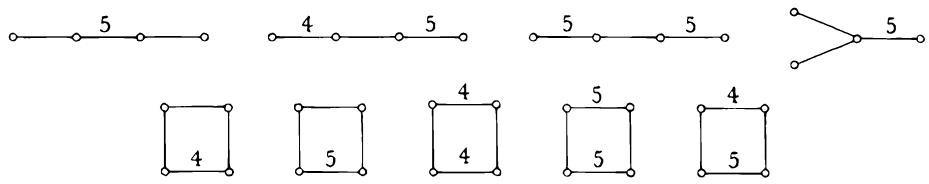
\includegraphics[keepaspectratio]{images/part001_8fab2eba.jpg}}

\begin{enumerate}
\def\labelenumi{\alph{enumi})}
\setcounter{enumi}{1}
\tightlist
\item
  对秩 5 回答同样的问题，其清单由下列五个图组成：
\end{enumerate}

\pandocbounded{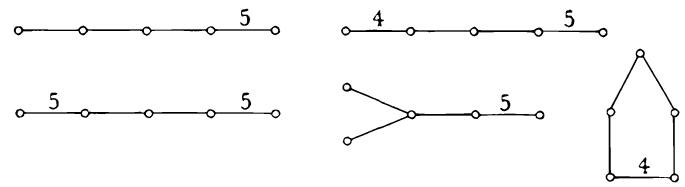
\includegraphics[keepaspectratio]{images/part001_6b3cac07.jpg}}

\begin{enumerate}
\def\labelenumi{\alph{enumi})}
\setcounter{enumi}{2}
\tightlist
\item
  证明不存在秩 \(\geqslant 6\) 的紧双曲型图。*
\end{enumerate}

\begin{enumerate}
\def\labelenumi{\arabic{enumi})}
\setcounter{enumi}{15}
\tightlist
\item
  *证明：任何有一条系数为 6 的棱的、秩 \(\geqslant 4\) 的双曲型 Coxeter 图都同构于下列十一个图之一（它们是非紧的且秩为 4）：
\end{enumerate}

\pandocbounded{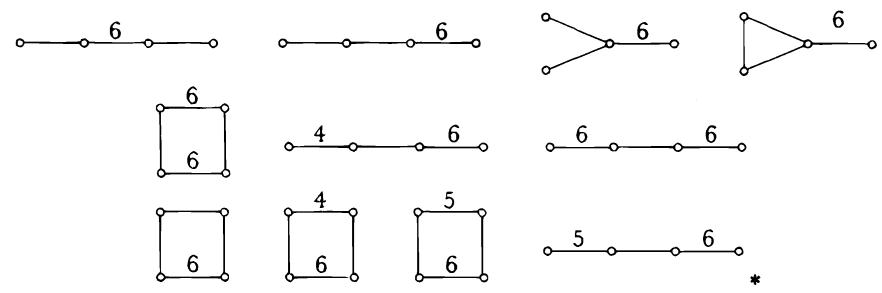
\includegraphics[keepaspectratio]{images/part001_2926a96c.jpg}}

\begin{enumerate}
\def\labelenumi{\arabic{enumi})}
\setcounter{enumi}{16}
\tightlist
\item
  *证明：更高秩的双曲 Coxeter 图是下列三个图（它们的秩为 10）：
\end{enumerate}

\pandocbounded{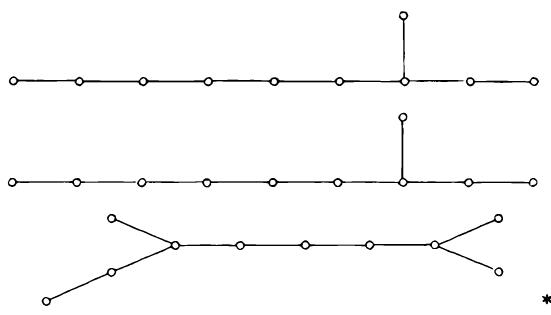
\includegraphics[keepaspectratio]{images/part001_3a8f46b0.jpg}}

¶ 18) 假设 (W,S) 是双曲型的，且 W 使 E 的一个格 \(\Gamma\) 稳定。设 G 是 \(B_{M}\) 的正交群，设 \(G(\Gamma)\) 是元素 \(g \in G\)（满足 \(g\Gamma = \Gamma\)）组成的子群。证明 \(G(\Gamma)\) 是 G 的离散子群。证明 W 是 \(G(\Gamma)\) 的有限指数子群（利用 W\textbackslash G 的测度有限这一事实）。

*若 (W, S) 实际上是紧双曲型的，证明相应的 Coxeter 图同构于下列图之一（使用 Exercs. 4, 6 与 15）：

\pandocbounded{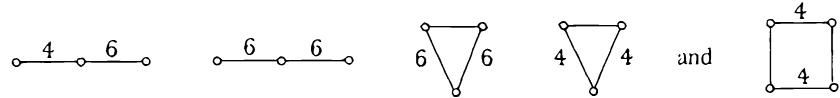
\includegraphics[keepaspectratio]{images/part001_0d92fd3d.jpg}}

证明与 Exerc. 16 的图（最后四个除外）相应的群都使一个格稳定（使用 Exerc. 6 的方法）。*

\begin{enumerate}
\def\labelenumi{\arabic{enumi})}
\setcounter{enumi}{18}
\tightlist
\item
  设 \((W,S)\) 是与图
\end{enumerate}

\pandocbounded{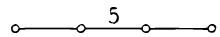
\includegraphics[keepaspectratio]{images/part001_8b3dcc37.jpg}}

相应的 Coxeter 系统。它是一个紧双曲型的系统（cf.~Exerc. 15）。型 \(B_{M}\) 关于基 \((e_{s})\) 的系数属于域 \(\mathbf{Q}(\sqrt{5})\) 中由该域的在 Z 上整的元素组成的子环 A。

\begin{enumerate}
\def\labelenumi{\alph{enumi})}
\item
  设 \(\sigma\) 是 \(K\) 到 \(\mathbf{R}\) 中的、把 \(\sqrt{5}\) 映为 \(-\sqrt{5}\) 的嵌入。证明 \(\sigma(B_M)\)（型 \(B_M\) 在 \(\sigma\) 下的像）非退化且正。
\item
  设 G 是 \(B_{M}\) 的正交群，\(G_{\sigma}\) 是 \(\sigma(B_{M})\) 的正交群。设 \(G_{A}\) 是 G 中由关于 \((e_{s})\) 的矩阵系数在 A 中的元素组成的子群。证明 \(G_{A}\) 可与 \(G \times G_{\sigma}\) 的一个离散子群等同，然后利用 a) 证明 \(G_{A}\) 是 G 的离散子群。
\item
  证明 W 是 \(G_{A}\) 的一个有限指数子群。
\end{enumerate}

\(d)\) 对 Exerc. 15 中的其余图证明类似的结果（域 \(\mathbf{Q}(\sqrt{5})\) 有时换成 \(\mathbf{Q}(\sqrt{2})\)），但下面的图除外：

\pandocbounded{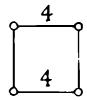
\includegraphics[keepaspectratio]{images/part001_99b486d1.jpg}}

即 Exerc. 18 中处理的图，以及图 \(^{8}\)

\pandocbounded{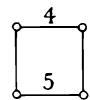
\includegraphics[keepaspectratio]{images/part001_2a5e784a.jpg}}

¶ 20) 对 S 的每个子集 \(\{s, s'\}\)（满足 \(m(s, s') = \infty\)），设 \(r(s, s')\) 是一个实数 \(\leqslant -1\)。给 E 赋以双线性型 \(\mathbf{B}_r\)，使得

\[
\begin{array}{l l} \mathrm{B} _ {r} (e _ {s}, e _ {s ^ {\prime}}) = \mathrm{B} _ {\mathrm{M}} (e _ {s}, e _ {s ^ {\prime}}) = - \cos \frac {\pi}{m (s , s ^ {\prime})} & \text {if} m (s, s ^ {\prime}) \neq \infty \\ \mathrm{B} _ {r} (e _ {s}, e _ {s ^ {\prime}}) = r (s, s ^ {\prime}) & \text {if} m (s, s ^ {\prime}) = \infty . \end{array}
\]

与 \(B_{M}\) 的情形一样，我们定义反射 \(\sigma_{s}\)，它以 \(e_{s}\) 为向量，且使型 \(B_{r}\) 不变。

\begin{enumerate}
\def\labelenumi{\alph{enumi})}
\item
  证明存在唯一的同态 \(\sigma_r: \mathbf{W} \to \mathbf{GL}(\mathbf{E})\)，使得 \(\sigma_r(g_s)\) 等于上面定义的反射 \(\sigma_s\)。
\item
  证明 Prop. 4、Th. 1 及其诸系、以及 Lemma 1 中的断言对 \(\sigma_r\) 仍然成立。
\end{enumerate}

